\documentclass[journal, a4paper]{IEEEtran}

%\usepackage{cite}
\usepackage{graphicx}
%\usepackage{psfrag}
%\usepackage{subfigure}
\usepackage{url}
%\usepackage{stfloats}
\usepackage{amsmath}
%\usepackage{array}

% Package Settings
\graphicspath{ {images/} }

\begin{document}

% Define document title and author
    \title{Testing the Effects of Transfection on Mammalian Cytokine RNA Expression}
    \author{Austin Mitchell Vecchio
    \thanks{Advisor: Dipl.--Ing.~Michelle Ammerman, Lehrstuhl f\"ur Nachrichtentechnik, TUM, WS 2050/2051.}}
    \markboth{Hauptseminar Digitale Kommunikationssysteme}{}
    \maketitle

% Write abstract here
\begin{abstract}
  Abstract outline


  This experiment aims to study the effect of genetic expression on polyplex treated cells against $\beta$-actin and INF$\alpha$.

\end{abstract}

% Each section begins with a \section{title} command
\section{Introduction}
    \PARstart{T}{his} section introduces the topic and leads the reader on to the main part.

    Real Time PCR
      Generate large quantity of DNA from cDNA templates. Can view amount of DNA in each cycle.
      Can be seen if immunological response was indicated.

      There are multiple controls used throughout this experiment. For controls that compare directly against the immunological
      transcripts $\beta$-actin and RPL13A will be used. INF$\beta$ will not be used as it will only appear after cycle 40 in the experiment producing undesirable results.
      The No Template Control will consist of DEPC water.

    Outline

      polyplex polycationic
      treatments
      samples
      form an immune response
    The mRNA sampl

Test the effects on

Each student was given a sample as follows

 IL6 and IFN$\alpha$ are used as the immunilogical transcripts
DEPC water is the no template control

Poly24 Av
Poly24 Ts
Just Cells
No Wash

It is virtually impossible to completely eliminate all genomic DNA from RNA preparations. Therefore, if the assay is not cDNA-specific, it is important to include a minus-reverse transcriptase ("-RT") control in real-time RT-PCR experiments. Typically, the "-RT" control is a mock reverse transcription containing all the RT-PCR reagents, except the reverse transcriptase. The presence of an amplification product in the "-RT" control is indicative of contaminating DNA in the sample.”

% Main Part
\section{Methods}
    \subsection{Purification}
      The cells in trizol were thawed before phase separation. During phase separation,
      the poly treated cells in trizol were incubated for a duration of 5 minutes. An addition of chloroform was then added
      to the homoginized sample according to the ratio of 0.2mL of chloroform was added for every 1mL of Trizol reagent.
      The homoginized sample was incubated following a vigorous shake. The sample was then centrifuged for 15 min and the aqueous phase
      was removed and stored in a second tube. Isopropanol was added to the aqueous phase at a ratio of 0.5$\mu$L of isopropanol per 1$\mu$ of Trizol.
      Solution was centrifuged for 20 min and remove ethanol leaving only the pellet. Resuspend pellet in RNase free water. Incubate in heat block at 42C for 10-15 min.

    \subsection{cDNA Synthesis}

        \begin{table}[!hbt]
          % Center the table
          \begin{center}
          \caption{cDNA Concentrations}
          \label{tab:simParameters}
          \begin{tabular}{|c|c|}
            \hline
            +RT & -RT \\
            \hline
            1$\mu$L 10x dsDNase Buffer & 10x 1$\muu$L 10x dsDNase Buffer \\
            \hline
            1$\mu$L dsDNase & 1$\muu$L dsDNase \\
            \hline
            1$\mu$L Template RNA & 1$\muu$L Template RNA \\
            \hline
            2$\mu$L Total RNA (Poly24) & 2$\muu$L Total RNA (Poly24) \\
            \hline
          \end{tabular}
          \end{center}
        \end{table}

        \begin{table}[!hbt]
          % Center the table
          \begin{center}
          \caption{cDNA Concentrations}
          \label{tab:simParameters}
          \begin{tabular}{|c|c|}
            \hline
            +RT & -RT \\
            \hline
            4$\mu$L 5x Reaction Mix & 4$\mu$L 5x Reaction Mix \\
            \hline
            2$\mu$L Maxima Enzyme Mix & 2$\mu$L DEPC H20 \\
            \hline
            4$\mu$L Nuclease Free Water & 4$\mu$L Nuclease Free Water \\
            \hline
          \end{tabular}
          \end{center}
        \end{table}

    \subsection{Qt PCR}

      iTaq universal SYBR Green supermix 20&\mu&L Reaction
      10
      Permuation of Green supermix with four<> in a 2:1 ratio.
      5 microliters and 10 microliters.

      \begin{table}[!hbt]
        % Center the table
        \begin{center}
        \caption{cDNA Concentrations}
        \label{tab:simParameters}
        \begin{tabular}{|c|c|c|}
          \hline
          INFA & (Ts, AV, Mi) & 1.32 \\
          \hline
          INFA & (Ni) & 11.79 \\
          \hline
          $\beta$-Actin & (Ts, AV, Mi) & 2.00 \\
          \hline
          $\beta$-Actin & (Ni) & 2.9 \\
          \hline
        \end{tabular}
        \end{center}
      \end{table}

      Each well will get 6$\mu$L of 4ng/$\mu$L of dna as per.
      The concentrations of cDNA for Ts, Av and Mi were all around 100ng/ $\mu$ L. Therefore one set of calculations can be used for all three
      experiments. The concentrations of Ni, however, were reported ot be 11.2ng/ $\mu$ L and thus, had to have a different set of calculations.

      Adding supermix, following charts from above and water makex mix.

      The QPCR was ran for 40 cycles.

    \subsection{Gel Electrophoresis}

    \subsection{Analysis}
        Used $\Delta$\Delta$ct method was used in calculating fold inductions.

\section{Results}

  \subsection{Qubit}
    \begin{table}[!hbt]
      % Center the table
      \begin{center}
      % Fold Inductions
      \caption{Qubit Results}
      \label{tab:simParameters}
      % Table itself: here we have two columns which are centered and have lines to the left, right and in the middle: |c|c|
      \begin{tabular}{|c|c|}
      \hline
      SD1 & 54.27 \\
      \hline
      SD2 & 1057.52 \\
      \hline
      Tk & 8.75 \\
      \hline
      DA & 68.0 \\
      \hline
      AV & 487.0 \\
      \hline
      Tk & 28.0 \\
      \hline
      \end{tabular}
      \end{center}
    \end{table}

\section{Discussion}

For a future experiment, it would be suggested that the polyplex cells are treated in 3 hour increments from 3 hours to 24 hours.

\section{Conclusion}
The mRNA was purified and converted to cDNA. THe resulting concentration was relatively high compared to peers. This eludes that the
treatment for these cells of polycationic DNA for 24 hours could result in higher transcription rates.

\section{Figures}

  \begin{itemize}
    \item Columns 1-3 IL6
    \item Columns 4-6 INF$\alpha$
    \item Columns 7-9 $\beta$-acting
    \item Columns 10-12 RPL13A
  \end{itemize}

  \begin{table}[!hbt]
    % Center the table
    \begin{center}
    % Fold Inductions
    \caption{Wells for Immunological Responses}
    \label{tab:simParameters}
    % Table itself: here we have two columns which are centered and have lines to the left, right and in the middle: |c|c|
    \begin{tabular}{|c|c|c|c|c|c|c|c|c|c|c|c|c|}
      \hline
      & 1 & 2 & 3 & 4 & 5 & 6\\
      \hline
      A & 4ng/$\mu$L & 4ng/$\mu$L & 4ng/$\mu$L & 4ng/$\mu$L & 4ng/$\mu$L & 4ng/$\mu$L\\
      \hline
      B & 4ng/$\mu$L & 4ng/$\mu$L & 4ng/$\mu$L & 4ng/$\mu$L & 4ng/$\mu$L & 4ng/$\mu$L\\
      \hline
      C & 4ng/$\mu$L & 4ng/$\mu$L & 4ng/$\mu$L & 4ng/$\mu$L & 4ng/$\mu$L & 4ng/$\mu$L\\
      \hline
      D & 4ng/$\mu$L & 4ng/$\mu$L & 4ng/$\mu$L & 4ng/$\mu$L & 4ng/$\mu$L & 4ng/$\mu$L\\
      \hline
      E & Ts & Ni & AV & Ts & Ni & AV\\
      \hline
      E & Ts & Ni & AV & Ts & Ni & AV\\
      \hline
      G & Mi -RT & Mi NTC & & Mi -RT & Mi NTC & \\
      \hline
      H & & & & & &\\
      \hline
    \end{tabular}
    \end{center}
  \end{table}

%Tasha (Ts) Poly24
%Micah (Mi) No Wash
%Nick (Ni) Just Cells
%Austin (AV) Poly24
%-rt controls
%NTC


  \begin{table}[!hbt]
    % Center the table
    \begin{center}
    % Fold Inductions
    \caption{Wells for Controls}
    \label{tab:simParameters}
    % Table itself: here we have two columns which are centered and have lines to the left, right and in the middle: |c|c|
    \begin{tabular}{|c|c|c|c|c|c|c|c|c|c|c|c|c|}
      \hline
      & 7 & 8 & 9 & 10 & 11 & 12 \\
      \hline
      A & 4ng/$\mu$L & 4ng/$\mu$L & 4ng/$\mu$L & 4ng/$\mu$L & 4ng/$\mu$L & 4ng/$\mu$L\\
      \hline
      B & 4ng/$\mu$L & 4ng/$\mu$L & 4ng/$\mu$L & 4ng/$\mu$L & 4ng/$\mu$L & 4ng/$\mu$L\\
      \hline
      C & 4ng/$\mu$L & 4ng/$\mu$L & 4ng/$\mu$L & 4ng/$\mu$L & 4ng/$\mu$L & 4ng/$\mu$L\\
      \hline
      D & 4ng/$\mu$L & 4ng/$\mu$L & 4ng/$\mu$L & 4ng/$\mu$L & 4ng/$\mu$L & 4ng/$\mu$L\\
      \hline
      E & Ts & Ni & AV & Ts & Ni & AV\\
      \hline
      E & Ts & Ni & AV & Ts & Ni & AV\\
      \hline
      G & Mi -RT & Mi NTC & & Mi -RT & Mi NTC & \\
      \hline
      H & & & & & &\\
      \hline
    \end{tabular}
    \end{center}
  \end{table}

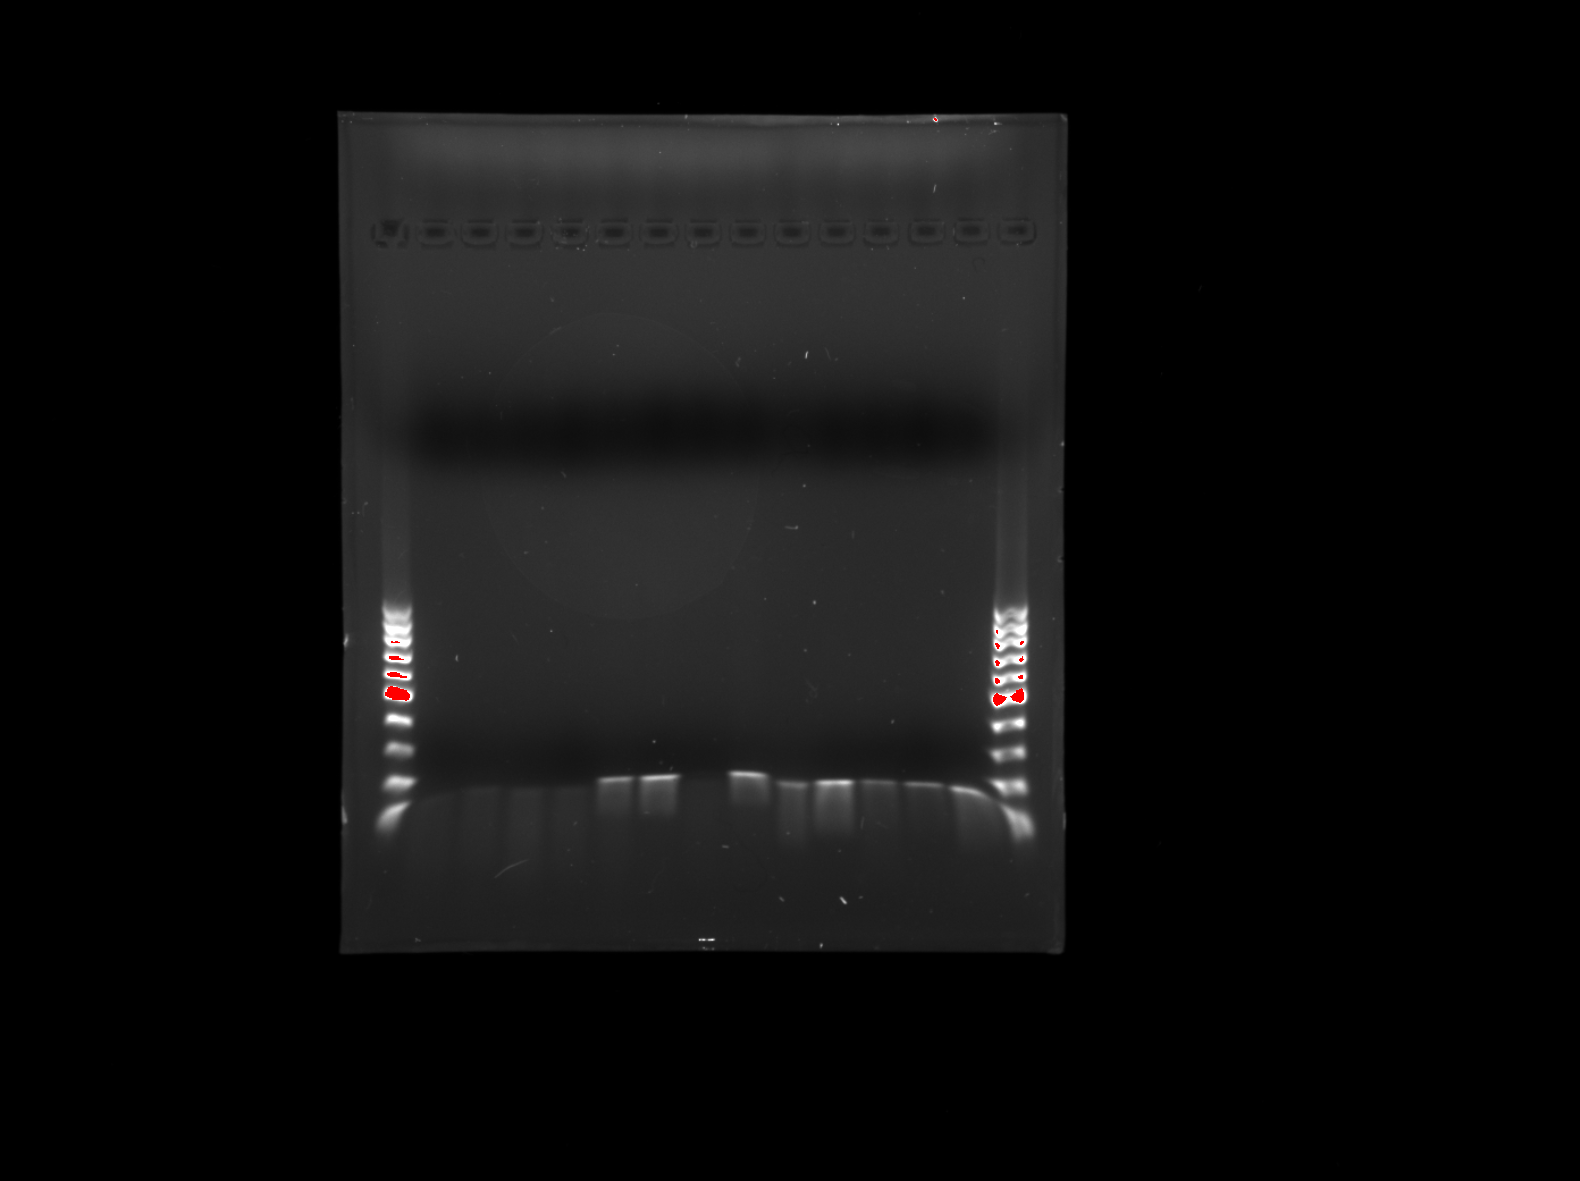
\includegraphics{gel.tif}

% Now we need a bibliography:
\begin{thebibliography}{5}
    %Each item starts with a \bibitem{reference} command and the details thereafter.
    \bibitem{HOP96} % Transaction paper
    J.~Hagenauer, E.~Offer, and L.~Papke. Iterative decoding of binary block
    and convolutional codes. {\em IEEE Trans. Inform. Theory},
    vol.~42, no.~2, pp.~429–-445, Mar. 1996.

    \bibitem{MJH06} % Conference paper
    T.~Mayer, H.~Jenkac, and J.~Hagenauer. Turbo base-station cooperation for intercell interference cancellation. {\em IEEE Int. Conf. Commun. (ICC)}, Istanbul, Turkey, pp.~356--361, June 2006.

    \bibitem{Proakis} % Book
    J.~G.~Proakis. {\em Digital Communications}. McGraw-Hill Book Co.,
    New York, USA, 3rd edition, 1995.

    \bibitem{talk} % Web document
    F.~R.~Kschischang. Giving a talk: Guidelines for the Preparation and Presentation of Technical Seminars.
    \url{http://www.comm.toronto.edu/frank/guide/guide.pdf}.

    \bibitem{5}
    IEEE Transactions \LaTeX and Microsoft Word Style Files.
    \url{http://www.ieee.org/web/publications/authors/transjnl/index.html}

\end{thebibliography}

% Your document ends here!
\end{document}
